\documentclass[conference]{IEEEtran}
\pagestyle{plain}

\usepackage[T1]{fontenc}
\usepackage[scaled=0.8]{beramono} % For a pretty monospaced font.
\usepackage[pdftex]{graphicx}
\usepackage{booktabs} % For pretty tables.
\usepackage{multirow} % Also for pretty tables.
\usepackage{xcolor} % For colourful links.
\usepackage{xspace} % For reasonable spacing in custom commands.
\usepackage[pagebackref=true]{hyperref} % For clickable links.
\usepackage{balance} % Balance columns on last page.
\usepackage{wasysym} % For \Circle, ...
\usepackage{listings} % For source code listings.
\usepackage{ifthen}
\usepackage[tight,footnotesize]{subfigure}

% Add custom text right before backreferences in literature.
\renewcommand*{\backref}[1]{}
\renewcommand*{\backrefalt}[4]{
   \ifcase #1
      No cited.
   \or
      (Cited on p.~#2)
   \else
      (Cited on pp.~#2)
   \fi}

\definecolor{darkblue}{rgb}{0,0,0.5}
\definecolor{lightgray}{rgb}{0.93,0.93,0.93}

\lstset{
	backgroundcolor=\color{lightgray},
	basicstyle=\footnotesize\ttfamily,
	keepspaces=true,
	breakatwhitespace=true,
	breaklines=true,
	numbers=left,
	numbersep=3pt,
	numberstyle=\scriptsize\color{gray},
}

\hypersetup{
	pdftitle={FingerprinTor: DNS Fingerprinting Attacks on Tor},
	pdfauthor={Anonymous},
	pdfkeywords={Tor, DNS, traffic correlation, anonymity},
	colorlinks=true,
	urlcolor=darkblue,
	linkcolor=darkblue,
	citecolor=darkblue
}

\newcommand{\xxx}[1]{\textcolor{red}{#1}}
\newcommand{\fixme}[1]{\textcolor{red}{{\bf FIXME:} #1}\xspace}
\newcommand{\ie}{{\it i.e.}\xspace}
\newcommand{\eg}{{\it e.g.}\xspace}
\newcommand{\ea}{{\it et al.}\xspace}
\newcommand{\etc}{{\it etc.}\xspace}
\newcommand{\first}{(\emph{i})\xspace}
\newcommand{\second}{(\emph{ii})\xspace}
\newcommand{\third}{(\emph{iii})\xspace}
\newcommand{\fourth}{(\emph{iv})\xspace}
\newcommand{\fifth}{(\emph{v})\xspace}

\newcommand{\name}{FingerprinTor\xspace}


\newcommand{\TABLECAPTIONS}{top} % "top" or "bottom". Silly IEEE formatting
\newcommand{\tabcaptext}{}
\ifthenelse{\equal{\TABLECAPTIONS}{top}}{%
\newcommand{\topcap}[1]{\caption{#1}}
\newcommand{\bottomcap}[1]{}
}
{
\newcommand{\topcap}[1]{}
\newcommand{\bottomcap}[1]{\caption{#1}}
}

\makeatletter
\def\blfootnote{\xdef\@thefnmark{}\@footnotetext}
\makeatother

\begin{document}

\title{FingerprinTor: DNS Fingerprinting Attacks on Tor}

\author{
\IEEEauthorblockN{Benjamin Greschbach$^*$}
\IEEEauthorblockA{KTH Royal Institute of Technology}
\and
\IEEEauthorblockN{Tobias Pulls$^*$}
\IEEEauthorblockA{Karlstad University}
\and
\IEEEauthorblockN{Laura M.  Roberts$^*$}
\IEEEauthorblockA{Princeton University}
\and
\IEEEauthorblockN{Philipp Winter$^*$}
\IEEEauthorblockA{Princeton University}
\and
\IEEEauthorblockN{Nick Feamster}
\IEEEauthorblockA{Princeton University}
}

% \IEEEoverridecommandlockouts
% \makeatletter\def\@IEEEpubidpullup{9\baselineskip}\makeatother
% \IEEEpubid{\parbox{\columnwidth}{Permission to freely reproduce all or part
%     of this paper for noncommercial purposes is granted provided that
%     copies bear this notice and the full citation on the first
%     page. Reproduction for commercial purposes is strictly prohibited
%     without the prior written consent of the Internet Society, the
%     first-named author (for reproduction of an entire paper only), and
%     the author's employer if the paper was prepared within the scope
%     of employment.  \\
%     NDSS '16, 21-24 February 2016, San Diego, CA, USA\\
%     Copyright 2016 Internet Society, ISBN 1-891562-41-X\\
%     http://dx.doi.org/10.14722/ndss.2016.23xxx
% }
% \hspace{\columnsep}\makebox[\columnwidth]{}}

\maketitle

\begin{abstract}
Previous correlation attacks on the Tor network have focused solely on
the attacks that are possible from analyzing a single TCP connection between
a client and a server. In reality, of course, a client application opens
several TCP connections to handle a single application request; many of
those TCP connections are also accompanied by DNS requests and
responses. This additional traffic presents many more opportunities for
an adversary to launch a correlation attack.
%
This paper quantifies the effects of DNS traffic on Tor users' anonymity.
We investigate how DNS can make existing attacks more powerful, as well
as how DNS lookups can leak information to third parties about anonymous
communication. We \first develop a
method to identify the DNS resolvers of Tor exit relays; \second show how
existing website fingerprinting (WF) attacks are stronger when they incorporate DNS
traffic; \third analyze the Internet-scale effects of these new attacks on Tor
users; and \fourth present an improved method to evaluate correlation
attacks.
%
We find that Google's DNS resolver observes almost 40\% of all DNS
requests exiting the Tor network. DNS requests also often traverse ASes
that the corresponding TCP connections do not transit, enabling
additional ASes to gain information about Tor users' traffic.
%%% 
\xxx{Abstract is very unclear from here down.}
By correlating the output of WF
attacks with observed DNS requests, WF+DNS attacks are perfectly precise for
unpopular websites, further motivating the introduction of WF defenses in Tor.
\fixme{Add insights about TorPS simulations.}
Finally, some of our findings generalize to other anonymity networks.
\end{abstract}


\blfootnote{$^*$All four authors contributed substantially, and share first authorship.}

\section{Introduction}
\label{sec:introduction}

% High-level motivation.
We have yet to learn how to build anonymity networks that
resist global adversaries, provide low latency, and scale well.  Remailer
systems such as Mixmaster~\cite{mixmaster} and
Mixminion~\cite{Danezis2003a} eschew low latency in favor of
strong anonymity.
In contrast, Tor~\cite{dingledine2004a} trades off strong anonymity to
achieve low latency; Tor therefore
enables latency-sensitive applications such as web browsing but is
vulnerable to
adversaries that can observe traffic both
entering and exiting its network, thus enabling deanonymization.
Although Tor does not consider global adversaries in its threat model,
adversaries that can observe traffic for extended periods of time in
multiple network locations (\ie, ``semi-global'' adversaries) are a real
concern~\cite{Farrell2014a,Johnson2013a}; we need to better understand
the nature to which these adversaries exist in operational networks and
their ability to deanonymize users.

% More specific problem.
Past work has quantified the extent to which an adversary that
observes TCP flows between clients and servers (\eg, HTTP requests,
BitTorrent connections, and IRC sessions) can correlate traffic flows
between the client and the entry to the anonymity network and between
the exit of the anonymity network and its ultimate
destination~\cite{Johnson2013a,Murdoch2007a}. The ability to correlate
these two flows---a so-called {\em correlation attack}---can link the
sender and receiver of a traffic flow, thus compromising the anonymity
of both endpoints. Although TCP connections are an important part
of communications, the Domain Name System (DNS) traffic is also
quite revealing: for example, even loading a single webpage can generate
hundreds of DNS requests to many different domains. No previous analysis
of correlation attacks has studied how DNS traffic can exacerbate
these attacks.

DNS traffic is highly relevant for correlation attacks because it
often traverses completely different paths
and autonomous systems (ASes) than the subsequent corresponding TCP
connections.  An attacker that can observe occasional DNS
requests may still be able to link both ends of the communication, even
if the attacker cannot observe TCP traffic between the exit of the
anonymity network and the server.
Figure~\ref{fig:overview} illustrates how an adversary may
monitor the connection between a user and the guard relay, and between the exit
relay and its DNS resolvers or servers.  This
territory---to-date, completely unexplored---is the focus of this work.

\begin{figure}[t]
	\centering
	
\includegraphics[width=0.65\linewidth]{figures/attack-concept.pdf}
	\caption{Past traffic correlation studies have focused on linking the TCP
		stream entering the Tor network to the one(s) exiting the network.  We
		show that an adversary can also link the associated DNS traffic, which
		can be exposed to many more ASes than the TCP stream.}
	\label{fig:overview}
\end{figure}

% Summary of our paper.
We first explore how Tor exit relays resolve DNS names.  By developing a new
method to identify all exit relays' DNS resolvers, we learn that Google
currently sees almost 40\% of all DNS requests exiting the Tor network.  Second,
we investigate which organizations can observe DNS requests that originate from
Tor exit relays.  To answer this question, we emulate DNS resolution for the
Alexa Top 1,000 domains from an autonomous system that is popular among exit
relays.  We find that DNS resolution for half of these domains traverses numerous
ASes that are not traversed for the subsequent HTTP connection to the web site.
We further introduce a new method to perform traceroutes from the networks where
exit relays are located, making our results significantly more accurate and
comprehensive than previous work.  Next, we show how the ability to observe DNS
traffic from Tor exit relays can augment existing website fingerprinting
attacks, yielding perfectly precise \name\footnote{The acronym is short for
\underline{D}NS-\underline{e}nhanced \underline{f}ingerprinting and
\underline{e}gress \underline{c}orrelation on \underline{Tor}.} attacks for
unpopular websites.  Finally, we use the Tor Path Simulator (TorPS)~\cite{TorPS}
to investigate the effects of Internet-scale \name attacks.

% Comparison to past work.
We demonstrate that DNS requests significantly increase the opportunity
for adversaries to perform correlation attacks. This finding should
encourage future work on correlation attacks to consider both TCP
traffic and the corresponding DNS traffic; future design decisions
should also be cognizant of this threat.  The measurement methods we use
to evaluate the effects of traffic correlation attacks are also more
accurate than past work. Our work \first serves as guidance to Tor exit
relay operators and Tor network developers, \second improves
state-of-the-art measurement techniques for analysis of correlation attacks, and \third
provides even stronger justification for introducing website fingerprinting defenses in
Tor.  To foster future work and facilitate the replication of
our results, we publish both our code and datasets.\footnote{Our project page is
available at \url{https://nymity.ch/tor-dns/}.}
In summary, we make the following contributions:
\begin{itemize}

\item We show how existing website fingerprinting attacks can be
  augmented with observed DNS requests by an AS-level adversary to
  yield perfectly precise \name attacks for unpopular websites.

\item We develop a method to identify the DNS resolver of exit
  relays. We find that Tor exit relays comprising 40\% of Tor's exit
  bandwidth rely on Google's public DNS servers to resolve DNS queries.

\item We quantify the extent to which DNS resolution exposes Tor users
  to additional AS-level adversaries who are not on the path between the
  sender and receiver.  We find that for the Alexa top 1,000 most
  popular websites, 60\% of the ASes that are on the paths between the
  exit relay and the DNS servers required to resolve the sites' domain
  names are not on the path between the exit relay and the website.

\item We develop a new measurement method to evaluate the extent to
  which ASes are on-path between exit relays and DNS resolvers. We use
  the RIPE Atlas~\cite{atlas} platform to achieve previously
  unprecedented path coverage and accuracy for evaluating the
  capabilities of AS-level adversaries.
\end{itemize}
\noindent
The rest of this paper is organized as follows.
Section~\ref{sec:background} presents background, and
Section~\ref{sec:related_work} relates our study to previous work.  In
Section~\ref{sec:landscape}, we shed light on the landscape of DNS in
Tor.  Section~\ref{sec:attack} discusses our \name attacks, which we
evaluate in Section~\ref{sec:analysis}.  We then model the
Internet-scale effect of our attacks in
Section~\ref{sec:internet-scale}.  Finally, we discuss our work in
Section~\ref{sec:discussion} and conclude the paper in
Section~\ref{sec:conclusion}.


\section{Background}
\label{sec:background}
We now give a brief introduction to the pillars our attack is resting
on---website fingerprinting and the process of DNS resolution over the Tor
network.

\subsection{Website fingerprinting attacks}
The Tor network encrypts relayed traffic as it travels from the client to the
exit relay.  Therefore, intermediate parties such as the user's Internet service
provider (ISP) are not able to read any packet content.  However, Tor does not
protect meta information such as data timing, frequency, and length.  Exploiting
these properties, the ISP can use a classifier to guess what sites the user is
visiting---despite Tor's encryption.  The literature calls this kind of attack a
\emph{website fingerprinting attack}.

Tor---and any other anonymity network---could eliminate website fingerprinting
attacks by employing leak-resistant, constant-rate channels between a Tor client
and its guard.  Unfortunately, the Tor network's limited spare capacity does not
allow for such an expensive defense, but some research has worked on making it
cheaper~\cite{Cai2014a}.

\subsection{How Tor handles DNS}
To preserve their anonymity and prevent DNS leakage, Tor clients must send their
DNS requests also over Tor.  Since Tor does not transport UDP packets, there is
a workaround to ensure that DNS requests go over Tor.

First, applications such as Tor Browser establish a connection to the SOCKS
proxy exposed by the local Tor client.  Using the SOCKS protocol, applications
instruct the Tor client to establish a circuit to a given domain and
port.\footnote{SOCKS in version 4a and 5 supports connection initiations using
domain names in addition to IP addresses.} The Tor client then selects an exit
relay whose exit policy matches the given domain and port.  Next, the client
sends a \texttt{BEGIN\_DIR} Tor cell to the exit relay, instructing it to
resolve the domain name and establish a TCP connection to the given port.  After
successfully establishing a connection, the exit relay responds with a
\texttt{RELAY\_CONNECTED} cell to the local Tor client.  From then on, data can
be exchanged with the intended destination.

As of Dec 2015, exit relays resolve domain asynchronously and both the exit
relay and the client maintain a caching layer around the resolution code to
speed up repeated lookups.  Exit relays send their DNS requests to the system
resolver, which is in \texttt{/etc/resolv.conf} on Linux systems.  The system
resolver is not set by Tor, and contains whatever the exit relay operator
configured, e.g., the ISP's resolver, or well-known, public resolvers such as
8.8.8.8.


\section{Related work}
\label{sec:related_work}
Our work combines traffic correlation with website fingerprinting attacks,
which is why we split related work into these two topics.

\paragraph{Traffic analysis methods}
Tor's threat model excludes global adversaries~\cite{Dingledine2004a}, but the
practical threat of such adversaries is an important question that academia has
spent considerable effort on answering.  In 2004, when the Tor network counted
only 33 relays, Feamster and Dingledine investigated the practical threat that
network-level adversaries pose to anonymity networks~\cite{Feamster2004a}.  In
particular, the authors considered an attacker that controls an autonomous
system that is traversed both for ingress and egress traffic, allowing the
attacker to correlate both streams.  Using AS path prediction~\cite{Gao2001a},
Feamster and Dingledine found that powerful tier-1 ISPs reduce location
diversity of anonymity networks.  In 2007, Murdoch and Zieli\'{n}ski drew
attention to IXP-level adversaries, a class of adversaries that was missing in
Feamster and Dingledine's work~\cite{Murdoch2007a}.  Murdoch and
Zieli\'{n}skishowed showed that IXP adversaries are able to correlate traffic
streams, even in the presence of packet sampling rates as low as one in 2,000.
In 2013, Johnson et al.~\cite{Johnson2013a} presented the first large-scale
study on the risk of Tor users facing relay-level and network-level
adversaries.  The authors developed a Tor path simulator (TorPS~\cite{TorPS})
that simulates Tor circuits for a number of user models the authors developed.
By combining TorPS with AS path prediction, Johnson et al. could answer
questions such as the average time until a Tor user's circuit is linked
together by an AS or IXP.  In 2015, Juen et al.~\cite{Juen2015a} questioned the
accuracy of path prediction algorithms that prior
work~\cite{Johnson2013a,Feamster2004a} used to estimate the threat of
correlation attacks.  The authors compared AS path predictions to millions of
traceroutes they initiated from 25\% of Tor relays by bandwidth at the AS
level.  Only 20\% of predicted paths matched the paths observed in traceroute,
calling into question the results of prior work.  A limitation of Juen et al.'s
work is that they could not consider the reverse path in traceroutes.  This
shortcoming was addressed in 2015 by Sun et al.~\cite{Sun2015a}.  While past
work treated routing as static, Sun et al.  leveraged the dynamic nature of
routing to show that network adversaries are a bigger threat than thought.
Most recently in 2016, Nithyanand et al.~\cite{Nithyanand2016a} used AS path
prediction to evaluate the practical threat faced by users in the top 10
countries using Tor.  We improve on previous work in two significant ways;
(\emph{i}) we are the first to consider the DNS protocol for traffic analysis
and evaluate its practical threat, and (\emph{ii}) we propose a method to scale
the measurement method proposed by Juen et al.~\cite{Juen2015a}.  Our method
leverages the volunteer-run RIPE Atlas measurement platform~\cite{atlas}
instead of convincing relay operators to run third-party scripts.  This allows
us to fully automate our method and achieve previously unprecedented scale.

\paragraph{Website fingerprinting}
In 2009, Hermann, Wendolsky, and Federrath~\cite{Hermann2009a} demonstrated the
first website fingerprinting attack against anonymity systems---including
Tor---in a closed-world setting.  In 2011, Panchenko et
al.~\cite{Panchenko2011a} greatly improved on Hermann et al.'s detection rate
and provided insight into an open-world setting.  In 2012, Cai et
al.~\cite{Cai2012a} improved on prior work by proposing an attack that used
Hidden Markov Models to determine if a sequence of page requests all come from
the same site.  The authors used an open-world setting for their evaluation.
Wang and Goldberg~\cite{Wang2013a} proposed an improved attack that employed a
new method for data gathering.  Instead of working with TCP segments, the
authors extracted Tor cells from packet traces and managed to remove flow
control cells from the traces.  In 2014, Wang et al.~\cite{Wang2014a} further
improved on their results.  Cai et al.~\cite{Cai2014b} analyzed what traffic
features provide the most predictive power, proved a lower bound of any defense
that achieves a certain level of security, and provided a framework to
investigate the performance of fingerprinting attacks.
Juarez~\cite{Juarez2014a} critically evaluated past fingerprinting attacks,
showing that they all made numerous simplifying assumptions.  The authors
suggest that fingerprinting attacks are still difficult to run outside a lab
setting as an attacker will have to consider operating system differences, page
changes, and background traffic.  Most recently in 2016, Panchenko et
al.~\cite{Panchenko2016a} showed that web\emph{page} fingerprinting lacks
precision in the open world while web\emph{site} fingerprinting remains
practical.  \fixme{What are we doing better than past work?}


\section{Understanding the Landscape}
\label{sec:landscape}

Before explaining our attack, we need to better understand how Tor performs DNS
resolution.  We begin by investigating how common it is for adversaries
to be able to observe DNS requests but \emph{not} subsequent TCP connections of
Tor users (Section~\ref{sec:as-exposure}).  We then seek to understand how
these results connect to the Tor network by determining the DNS resolvers used
by exit relays (Section~\ref{sec:mapping-resolvers}).

\subsection{Quantifying the additional AS exposure of DNS queries}
\label{sec:as-exposure}

Adversaries that can observe both DNS and subsequent TCP traffic (\eg, the ISP
of an exit relay) gain no benefit from seeing the client's DNS traffic,
since TCP traffic is sufficient to mount correlation
attacks~\cite{Murdoch2007a}.  In this work, we consider
adversaries that can observe traffic entering the Tor network and \emph{some}
DNS requests exiting the network---such as requests addressed to DNS
root servers---but {\em not} subsequent TCP traffic from exit relays.
We first determine the prevalence of these adversaries by measuring the
number of ASes that DNS queries traverse versus the
number of ASes subsequent web traffic traverses.

We quantify the {\em exposure} of DNS traffic versus TCP traffic as follows.  We
begin with Alexa's Top 1,000~\cite{alexatop1k}, a list of the 1,000 most popular
web sites as estimated by Alexa.  For each site, we conducted two
experiments.  First, we ran a TCP traceroute to the site, targeting port 80 to
mimic web traffic.  Second, we determined the DNS delegation path for the
website's DNS name using the {\tt dig} command's \texttt{+trace} feature.  The
delegation path of a domain name, say {\tt www.example.com}, is a hierarchy of
authoritative DNS servers, such as the authoritative server for {\tt .com}
pointing to the authoritative server for {\tt example.com}, which in turn points
to the authoritative server responsible for {\tt www.example.com}.  We also ran
UDP traceroutes to each server in the delegation path, targeting port 53 to
mimic DNS resolution.\footnote{The tool we developed for this purpose is
available online at \url{https://github.com/NullHypothesis/ddptr}.}
For both experiments, we then mapped all IP addresses in the traceroutes to AS
numbers~\cite{ipasn}, generating both a set of traversed ASes for DNS traceroutes
($\mathcal{D}$) and a set of traversed ASes for web traceroutes
($\mathcal{W}$).  Given these two sets for each of Alexa's Top
1,000, we compute the fraction of ASes that are \emph{only}
traversed for DNS traffic, but \emph{not} for web traffic ($\lambda$):

\begin{equation}
\label{equ:exposure}
\lambda \in [0, 1] =
\frac{|\mathcal{D} \setminus \mathcal{W}|}
     {|\mathcal{D} \cup \mathcal{W}|}.
\end{equation}
\noindent
The metric approaches 1 as the number of ASes that are only traversed for DNS
increases.  For example, if $\mathcal{D} = \{1,2,3\}$ and $\mathcal{W} =
\{2,3,4\}$, then $\lambda =
\frac{|\{1,2,3\} \setminus \{2,3,4\}|}{|\{1,2,3\} \cup \{2,3,4\}|} =
\frac{|\{1\}|}{|\{1,2,3,4\}|} =
\frac{1}{4} =
0.25$.  We determined $\lambda$ for each site in the Alexa Top 1,000 from five
autonomous systems in three countries.\footnote{The ASes are: OVH (France),
Gandi (France), Karlstad University (Sweden), Princeton University (U.S.), and
Comcast (U.S.).} One of our vantage points, the French OVH, is the most popular
AS by exit bandwidth as of August 2016.  It sees $10.98\%$ of exit traffic,
closely followed by AS 12876 (owned by the French Online) that sees $9.33\%$ of
exit traffic.  Our experiment consisted of 5,000 runs, 4,773 (95.5\%) of which
succeeded, and 227 (4.5\%) failed.

\begin{figure}[t]
	\centering
	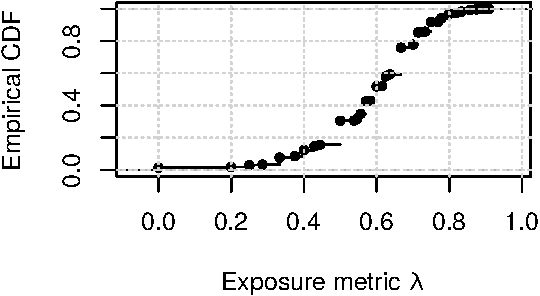
\includegraphics[width=0.75\linewidth]{figures/dns-exposure.pdf}
	\caption{Five box plots capturing the AS exposure metric $\lambda$ for
		Alexa's Top 1,000 web sites.  The box plots represent five autonomous
		systems in three countries.}
	\label{fig:exposure}
\end{figure}

The result is illustrated in Figure~\ref{fig:exposure}, which shows five box
plots capturing $\lambda$ values for Alexa's Top 1,000 sites.  The median of
all 4,773 $\lambda$ values is 0.571, so for half of all runs, DNS-only ASes
account for 57\% or more of all traversed ASes.  This result only applies to
exit relays that do their own DNS resolution; for relays that use a third-party
resolver, the ASes that are traversed between the exit relay and its DNS
resolver is the metric of interest.  We further believe that relays in regions
other than Western Europe or North America are likely to witness significantly
different exposure of DNS queries because many websites outsource their DNS
setup to providers such as CloudFlare whose points of presence are centered
around Western Europe and North America.  We conclude that adversaries that are
unable to observe a Tor user's TCP connection still have many opportunities to
see a TCP connection's corresponding DNS request.  Such adversaries include
(\emph{i}) popular open DNS resolvers such as Google and OpenDNS, (\emph{ii})
DNS root servers, and (\emph{iii}) network adversaries located on the path to
the previous two entities.

\subsection{Determining how Tor exit relays resolve DNS queries}
\label{sec:mapping-resolvers}

Having shown that the Internet provides ample opportunity for
AS-level adversaries to snoop on DNS traffic from exit relays, we
now investigate how the exit relays in the Tor network resolve DNS
queries in practice. Before this study,
we only had anecdotal evidence (\eg, from OpenDNS-powered error
messages~\cite[\S~4.1]{Winter2014b}) that some exit relays would occasionally
show.

We identify the DNS resolver of all exit relays by using {\tt
exitmap}~\cite{exitmap}, a scanner for Tor exit relays.  {\tt Exitmap} automates
running a task such as fetching a webpage over all one thousand exit relays,
making it possible to see the Internet through the ``eyes'' of every single exit
relay.  Using {\tt exitmap}, we resolve unique, relay-specific domains over each
exit relay, to a DNS server under our control.  Figure~\ref{fig:dnsenum}
illustrates this experiment.  To improve reliability, we configured {\tt
exitmap} to use two-hop circuits instead of the standard three-hop circuits.
The first hop was a guard relay under our control.  Over each exit relay, we
resolved a unique domain {\tt PREFIX.tor.nymity.ch}.  The prefix consisted of
the relay's unique 160-bit fingerprint, concatenated to a random 40-bit string
whose purpose is to prevent caching, so exit relays indeed resolve each query
instead of responding with a cached element.  We controlled the authoritative
DNS server of {\tt tor.nymity.ch}, so we could capture both the IP address and
packet content of every single query for {\tt tor.nymity.ch}.

\begin{figure}[t]
	\centering
	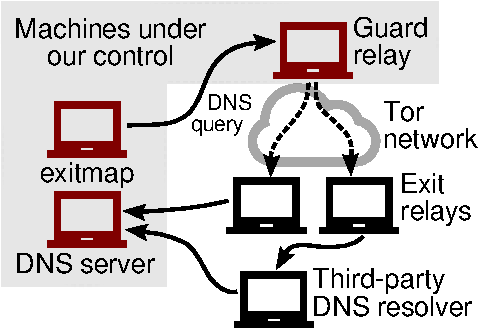
\includegraphics[width=0.6\linewidth]{figures/resolver-identification.pdf}
	\caption{Our method to identify the DNS resolvers of exit relays.  Over
	each exit relay, we resolve relay-specific domain names that are under our
	control.  Inspecting our DNS server logs, we can then identify the IP
	address of all exit relay resolvers.}
	\label{fig:dnsenum}
\end{figure}

An exit relay can either run its own resolver, as shown in the left exit relay in
Figure~\ref{fig:dnsenum}; or rely on a third-party resolver, such as the one
provided by its ISP, as shown in the right exit relay in Figure~\ref{fig:dnsenum}.  If
an exit relay runs its own resolver, we expect to receive a DNS request from
the exit relay's IP address, but if an exit relay uses a third-party resolver,
we expect to receive a request from an unrelated IP address.  Having encoded
relay-specific fingerprints in the query names, we are able to map queries to
exit relays in such cases.  We ran this experiment from September 2015 to May
2016, at least once a day.  Once we started to analyze our data, we identified
the following two challenges:

\begin{itemize}
\item {\em DNS proxies:}
We found that several exit relays used DNS
proxies---machines that passed on DNS requests to an actual resolver
instead of resolving it themselves.  Google's server {\tt 8.8.8.8} is a popular
example of a DNS proxy;
several dozen machines perform resolution in the
background~\cite{google-proxies}.  DNS proxies do
not interfere with our measurements, so we ignored them.

\item {\em Multiple DNS resolvers:}
On Linux systems, DNS resolution is controlled by the file
\texttt{/etc/resolv.conf}.  It contains a list of up to three DNS resolvers
that are queried in order.  If the primary resolver does not respond within a
time limit, the system falls back to the second, and finally the third
resolver.  Our data suggests that several exit relays used
different resolvers in subsequent {\tt exitmap} scans---one relay, for example,
used both Google's DNS resolver and one provided by its ISP.  For our
visualization, we only consider the first resolver we observed for an exit
relay, which might not be the primary resolver.
\end{itemize}
\noindent
Figure~\ref{fig:exit-resolvers} illustrates the fraction of DNS requests that
four of the most popular organizations could observe.  Google averages at 33\%,
but at times saw more than 40\% of all DNS requests exiting the Tor network---an
alarming number for a single organization.  Second to Google is ``Local''---exit
relays that run their own resolver, averaging at 12\%.  Next is OVH, which used
to be as popular as local resolvers, but slowly lost its share over time.  Note
that in contrast to Google, OVH does not run a public DNS server; the company's
resolvers are only accessible to its customers.  Finally, there is OpenDNS,
which also runs public DNS resolvers.  OpenDNS saw occasional spikes in
popularity but always remained in the single digits.  Apart from the illustrated
top resolver setups, the distribution has a long tail, presumably consisting of
many ISP resolvers.

\begin{figure*}[t]
	\centering
	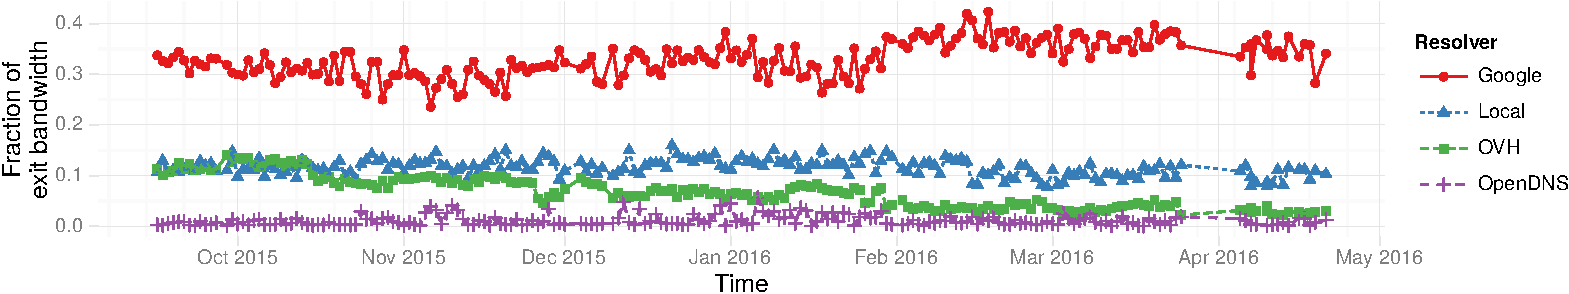
\includegraphics[width=\linewidth]{figures/asn-bw-frac.pdf}
	\caption{The popularity of some of the most popular DNS resolvers of exit
		relays over time.  The $y$ axis depicts the fraction of exit bandwidth
		that the respective resolver is responsible for.  Google's DNS resolver
		is by far the most popular, at times serving more than 40\% of all DNS
		requests coming out of the Tor network.  Google is followed by local
		resolvers, which average at around 12\%.  Once serving a fair amount of
		traffic, OVH dropped in popularity, and is now close to OpenDNS, an
		organization that runs an open resolver.}
	\label{fig:exit-resolvers}
\end{figure*}

% The following section takes up too much space, so it's commented out for now.
% We should include it in an extended version of our work, though.

\iffalse
\subsection{Inferring resolver configuration}
\label{sec:mapping-configuration}

In addition to identifying an exit relay's DNS resolver, our measurement
techniques can ascertain aspects of the of how an exit relay's local
resolver are configured.  It is important to identify broken resolvers
because they jeopardize the anonymity of Tor users.  Resolvers with poor
or broken configuration pose a security risk to Tor users as attackers
could poison or enumerate their cache, allowing them to redirect users
or profile them. Below, we discuss certain aspects of Tor's DNS resolver
configurations that we can infer with our measurements.

\paragraph{Random source ports}
To impede cache poisoning attacks, DNS resolvers should use random
source ports instead of always using UDP port 53.  Our measurements can
determine whether a given resolver randomizes its source ports.  We
classify a resolver as ``uses randomization'' if the source port does
not equal 53.  This method causes a small number of false positives
because a randomizing resolver could use port 53 simply by chance.  The
probability of that happening is only $\frac{1}{65535}$.

We found 135 DNS resolvers that did not use random source ports.  These
resolvers were located in the networks of Vodafone, Germany (95\%), MTNL, India
(4\%), and Cogent, U.S. (1\%).

\paragraph{0x20 encoding}
Resolvers can further reduce the chance of cache poisoning by employing
{\tt 0x20} encoding (\ie, randomizing the capitalization of domain
names).  For example, to resolve {\tt foo.com}, a resolver would send a
request for {\tt fOo.CoM}.  If the DNS response does not reflect the
randomly chosen capitalization, the resolver considers unauthentic.  We
classify a resolver as ``uses {\tt 0x20}'' if it has at least one
lowercase and one uppercase character.  Again, there is a chance of
false positives, which depends on the domain name length.  A {\tt
  0x20}-encoded domain name of $n$ characters (excluding periods) can be
all-uppercase or all-lowercase with probability $2 \cdot 0.5^n$.

We found 427 DNS resolvers that did not use 0x20 encoding for at least one
query.  The top five resolvers were located in the networks of Google, U.S.
(38\%), AT\&T, U.S. (22\%), Deutsche Telekom, Germany (7\%), Yandex, Russia
(7\%), OpenDNS, U.S. (4\%).

\paragraph{DNSSEC validation}
We can verify whether a resolver is validating DNSSEC-signed records by resolving a
domain whose signature is deliberately malformed; 
{\tt dnssec-failed.org} provides such a service.  A validating resolver
would not return an {\tt A} record while
a non-validating resolver would.  Therefore, we send an {\tt A} query {\tt dnssec-failed.org} via
all exit relays and check whether we receive an response
\fi


\section{\name Attacks}
\label{sec:attack}

As with conventional correlation attacks, an attacker must observe
traffic that is both entering and exiting
the Tor network; in contrast to threat models from previous work, we
incorporate DNS instead of only
TCP traffic.
Figure~\ref{fig:attack-scenario} illustrates our correlation attack; it requires the
following building blocks:
\begin{figure}[t]
	\centering
	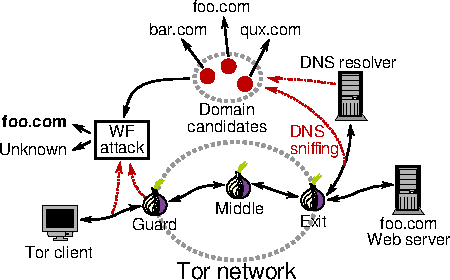
\includegraphics[width=0.8\linewidth]{figures/attack-scenario.pdf}
	\caption{An overview of the \name attack.  An adversary must monitor
		both ingress (encrypted Tor traffic) and egress (DNS request) traffic.
		A AS-level adversary between the
		client and its guard monitors ingress traffic.  The same adversary
		monitors egress traffic between the exit and a DNS server, or the DNS
		server itself.  Both ingress and egress traffic then serve as input to the
		\name attack.}
	\label{fig:attack-scenario}
\end{figure}

\begin{itemize}
    \item \emph{Ingress sniffing:} An attacker must observe traffic that is
		entering the Tor network.  The attacker can operate on the network level,
		as a malicious ISP or an intelligence agency.  In addition, the
		attacker can operate on the relay level by running a malicious Tor guard
		relay.  In both cases, the attacker can only observe encrypted
		data, so packet lengths and
		directions are the main inputs for website fingerprinting~\cite{Panchenko2016a}.
    \item \emph{Egress sniffing:} To observe both ends of the communication, an
		attacker must also observe egress DNS traffic.  We expect the adversary
		either to be on the path between exit relay
		and a DNS server or to run a malicious DNS
		resolver or server.  An attacker may also run an exit relay,
		but in this case conventional end-to-end correlation
		attacks~\cite{Murdoch2007a} are at least as effective as those we
		describe here.
\end{itemize}
We combine a conventional website fingerprinting attack operating on traffic
from ingress sniffing with
DNS traffic observed by egress sniffing, creating \name attacks. Our attacks
correlate the web\emph{sites} observed by the website fingerprinting attack in
ingress traffic with
the web\emph{sites} identified from DNS traffic. Next, we describe how we
simulate the DNS traffic from Tor exits, how we map DNS requests to websites,
and finally present our two \name attacks.

\subsection{Approximating DNS traffic from Tor exits}
\label{sec:attack:sim}

We first investigate the type and volume of DNS traffic that Tor's exit relays
send.  There are no logs of outgoing traffic
from Tor exit relays available to us, and ethical considerations kept us
from trying to collect them (\eg, by operating exit relays and recording
all the outgoing traffic). We therefore opt to approximate the DNS traffic
emerging from Tor exit relays by \first building a model of typical Tor
users' website browsing patterns, \second collecting a minimally invasive
dataset of DNS traffic, and \third accounting for the effects of DNS caching.

\subsubsection{Modeling which sites Tor users visit}
\label{sec:attack:pop}

We first build a model to approximate {which websites} Tor users visit.
As of July 2016, there are about 173 million active
websites~\cite{numberofwebsites}; the Alexa ranking~\cite{alexatop1k}
gives insights into their popularity based on the browsing behavior of
a sample of all Internet users. The distribution of the popularity of
these websites has previously been fit to a power-law distribution based
on the rank of the
website~\cite{Mahanti2013a,Clauset2009a,Ali2007a}.
For the pageview numbers of the Alexa top 10,000 websites, we found a
power-law distribution to be a good fit as neither a log-normal nor a
power-law distribution with exponential cutoff (\ie, a truncated power-law
distribution) offered significantly better fits.
We used the Python {\tt powerlaw} package~\cite{Alstott2014a} for fitting and
picked a power-law distribution with an $\alpha$ parameter of about $1.13$.
When varying the fitting parameter $x_{min}$ that determines beyond which
minimum value the power-law behavior should hold in the provided data, we can
get different $\alpha$ values. We made a conservative choice of picking this
smaller $\alpha$ value as it underestimates the popularity of popular websites
and therefore is worse for the attacker.\footnote{Alexa's page-view numbers
ignore multiple visits by the same user on the same day (see
\url{https://support.alexa.com/hc/en-us/articles/200449744}), so the ranking
might be slightly off when modeling website visit patterns.}
Thus, we use a power-law distribution to model what websites Tor users visit.
This might overestimate the popularity of higher-ranked websites such as
Facebook and YouTube because we believe that Tor users---who tend to be
privacy-conscious---are more likely to seek out alternatives than the typical
Internet user.  We will discuss the implications of our model for browsing
behavior later.

\subsubsection{Modeling how often Tor users visit each site}
\label{sec:load-freq}
% phw's numbers extrapolated
Next, we determine how many websites Tor users visit in a certain time span.
We approximated this number by setting up an exit relay whose exit policy
included only ports 80 and 443, so our relay would only forward web traffic.  We
then used the tool {\tt tshark} to capture the timestamps of DNS requests---but
no DNS responses.  We made sure that our {\tt tshark} filter did not capture
packet payloads or headers, so we were unable to learn what websites Tor users
were visiting.  In addition, we patched {\tt tshark} to log timestamps at a
five-minute granularity. The coarse timing granularity allows us to publish this
dataset with minimal privacy implications; Section~\ref{sec:ethics} discusses
the ethical implications of this experiment in more detail.  We ran the
experiment for approximately two weeks from May 15, 2016 to May 31, 2016, which
allowed us to determine the number of DNS requests for 4,832 five-minute
intervals.  Figure~\ref{fig:dns-reqs} shows this time series, but for clarity we
only plot May 25, 2016.  The distribution's median is 105, illustrated by the
red horizontal line.  The time series features several spikes; the most
significant one counts 1,410 DNS requests.  We repeated the same experiment with
the so-called \emph{reduced exit policy}\footnote{The reduced exit policy is
	available online at
\url{https://trac.torproject.org/projects/tor/wiki/doc/ReducedExitPolicy}.}
because it contains several dozen more ports and it is more popular among Tor
relay operators; as of August 2016, it is used by 7.8\% of exit relays by
capacity.  In comparison, the exit policy containing only port 80 and 443 only
accounts for 1.5\%.  The reduced exit policy resulted in a median of 102 DNS
requests per five minutes, so the difference between both policies is only three
DNS requests.

\begin{figure}[t]
	\centering
	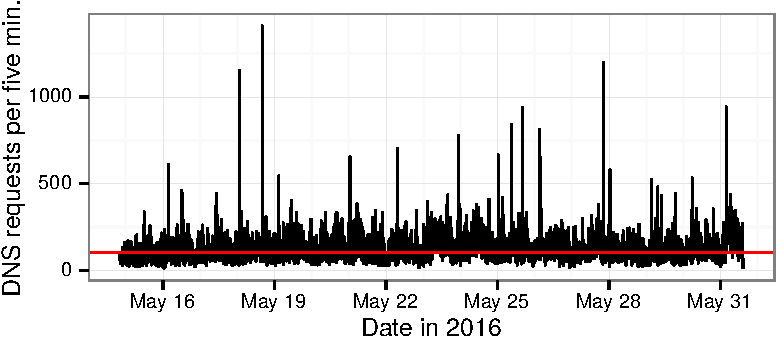
\includegraphics[width=\linewidth]{figures/dns-reqs.pdf}
	\caption{The number of DNS requests per five-minute interval on our
	exit relay for May 25, 2016.  Using a privacy-preserving measurement method,
	we only determined approximate timestamps and no content.  The red line at
	$y = 105$ illustrates the distribution median.}
	\label{fig:dns-reqs}
\end{figure}

We then interpolate these numbers to all Tor exit relays based on their
published bandwidth statistics.  While we measured a median of 105,
the mean of the distribution was 119.3 per five minutes during a two-week period.
From DNS statistics of the Alexa top one million websites (see
Section~\ref{sec:dns2site}) we know that one website visit causes outgoing DNS requests for 10.3 domains on average
(assuming a power-law distribution of site popularity as described above, and
taking into account Tor's caching of pending DNS requests, ensuring that multiple
requests sent by clients for the same domain name only result in one outgoing request
by the exit).
This means that we had an average of about 23.2 website visits per ten
minutes on our exit relay.  Assuming that the two main factors influencing the
volume of DNS requests are a relay's \emph{bandwidth} and \emph{exit policy},
and having shown that the exit policy does not significantly impact
the number of DNS requests, we can scale this number up to the whole Tor network
using the provided bandwidth of exit relays.  In particular, we use the
self-reported bandwidth information from Tor exit
relays collected in the so-called extra-info descriptors available on
CollecTor~\cite{collector}, and estimate the number of website visits on
each of the about 1,200 exit relays active at that time. The resulting average
total number of websites visited through the Tor network is about 536,000
websites per ten minutes.

Recently, Jansen and Johnson~\cite{Jansen2016a} measured the average
number of active web (port 80 and 443) circuits in Tor to about 700,000 per ten
minutes.\footnote{This number comes from a preprint kindly
shared by the authors and might change in the final version.}
Tor Browser, The Tor Project's fork of Firefox, builds one circuit per
website entered in the URL bar. How long the circuit remains active depends on
Tor Browser settings (primarily {\tt MaxCircuitDirtiness} currently set to ten
minutes) and how long TCP streams in the circuit are active: as long as at
least one stream is active, the circuit remains active.  Each time a new stream
is attached to a circuit, the circuit's dirtiness timeout is reset.
The number of active circuits serves as an
upper bound for the number of websites visited over Tor: visiting different
pages of a website will use the same circuit, and visiting a new website will
construct a new circuit.  Users visiting several pages of a website and websites
with long-lived reoccuring connections, like Twitter and Facebook with
continuously updating feeds,
all lower the number of websites visited in Tor relative to the number of active
circuits. In later sections we revisit the implications of our estimates by
scaling the Tor network to ten-times its estimated size.

\subsubsection{Modeling the effects of DNS caching at Tor exits}
To analyze which DNS requests the adversary can see, we need to
take caching of DNS responses into account. We ignore client-side DNS
caching since it is disabled by default, as described in
Section~\ref{sec:background}.
% From Tobias: I manually could not get Firefox to cache anything,
% not even between pageloads on the same site (went to kau.se, waited 20s,
% then clicked on a link: little tor client-side still got a DNS response
% from the exit for kau.se.)
On the exit relays, which perform DNS resolution on behalf of Tor clients,
caching is relevant because all Tor clients using the same exit relay share its
cache.  An exit relay maintains its own DNS cache%
\footnote{The code is available online at \url{https://gitweb.torproject.org/tor.git/tree/src/or/dns.c?id=tor-0.2.9.1-alpha}.}
(in addition to the cache of its DNS resolver) and enforces a minimum TTL of 60
seconds and a maximum TTL of 30 minutes.%
\footnote{The code is available online at \url{https://gitweb.torproject.org/tor.git/tree/src/or/dns.c?id=tor-0.2.9.1-alpha\#n209}.}
We refer to this as Tor's \emph{TTL clipping}. However, due to a bug in the
source code that we identified,%
\footnote{The bug report is available online at \url{https://bugs.torproject.org/19025}.}
the TTL of all DNS responses is set to 60 seconds.

If a Tor client attempts to resolve a domain that an exit relay already has in
its cache, the adversary will be unable to observe this request.  However, the
adversary can record all observed DNS requests over the past $x$
seconds, where $x$ is the maximum TTL value (\ie, maintain a sliding window of
length $x$).  If a Tor client
is attempting to resolve a domain name, the request is either cached or not.  If
it is not cached, the adversary will see it as a new, outgoing DNS request from
the exit relay. If it is cached, it must have been resolved by the exit relay in
the last $x$ seconds, and will therefore be in the sliding window.  The sliding
window technique allows the attacker to observe all DNS requests, regardless of
if they are cached or not at Tor exits.

We assume that an adversary applies this sliding window technique and models the
observable DNS data accordingly.  The attacker observes a fraction of Tor's exit
bandwidth for a specific window length, and together with our website visit
frequency estimation, this triggers a number of website visits in our
simulation.  For each visit event, we randomly draw a website using the
power-law website popularity distribution described above and put its DNS
requests into the window. As we will see next, we do not need to simulate or
consider the fact that the observed fraction of Tor exit bandwidth corresponds
to many different exits with individual caches.

\subsection{Inferring website visits from DNS requests}
\label{sec:dns2site}

Given a sliding window of DNS requests, we investigate how this information can
help determine whether a user has visited a website of interest.  In April 2016,
we visited the Alexa top one million websites five times, and collected all DNS
requests that each visit of a website's frontpage generated.  We refer to the
data collected for one visit as a \emph{sample}.  We performed these
measurements in five rounds from a university network, where each round browsed
all one million websites in a random order before visiting the same website
again. We used Tor Browser~5.5.4 and configured it {\em not to browse over Tor}:
Tor Browser ensures that the browser behavior is identical to a Tor Browser user
over Tor. By not using Tor, we can bypass IP blacklists and CAPTCHAs that are
triggered by IP addresses of exit relays~\cite{Khattak2016a}.
Table~\ref{tab:dns-censor} shows the percentage of websites in our dataset that
are hosted by CloudFlare or Akamai.  We might not be able to access these
websites programatically over Tor as they block or filter exit relays, as
identified by Khattak \ea~\cite{Khattak2016a}. We also include Google, which is
prevalent in our dataset and restricts access to Tor users for Google's search.

\begin{table}[t]
	\renewcommand{\tabcaptext}{The percentage of websites on Alexa top-1 million websites using providers
	involved in censoring or restricting access from
        Tor~\protect\cite{Khattak2016a}.}
      \topcap{\tabcaptext}
	\centering
	\begin{tabular}{l r}
	\toprule
	\textbf{Description} & \textbf{Percentage} \\
	\midrule
	Website behind CloudFlare IP & 6.44 \\
	Domain on website uses CloudFlare & 25.81 \\
	Domain on website uses Akamai & 33.86 \\
	Domain on website uses Google & 77.43 \\
	\bottomrule
	\end{tabular}
        \bottomcap{\tabcaptext}
	\label{tab:dns-censor}
\end{table}

We collected 2,540,941 unique domain names from a total of 60,828,453 DNS
requests. The dataset contains 2,260,534 domains that are unique to a particular
website, \ie, are not embedded on any other top million site; we call these
domains {\em unique domains}. Unique domains are particularly interesting
because they reveal to the adversary what sites among the top million the user
has visited.  This is not possible for domains such as {\tt youtube.com}, simply
because many websites embed YouTube videos.  Figure~\ref{fig:unique-domains}
shows the fraction of sites with unique domains for websites up to Alexa's top
one million.  We grouped all domains into 1,000 consecutive, non-overlapping
bins of size 1,000.  For 96.8\% of all sites on the Alexa top one million there
exists at least one unique domain.  Interestingly, more popular websites are
less likely to have a unique domain associated with them: only 77\% of the first
bin---the most popular 1,000 domains---contain at least one unique domain,
significantly less than the rest of the data.

Table~\ref{tab:dns-domains} shows summary statistics for the number of domains
per website. At least half of the sites have ten domains per website, two of
them are unique, suggesting that an adversary can identify many website visits
by observing a single unique DNS request.

\begin{figure}[t]
	\centering
	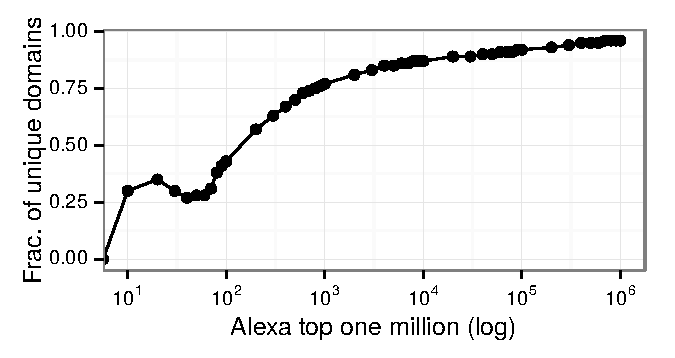
\includegraphics[width=0.75\linewidth]{figures/dns-unique-domains.pdf}
	\caption{The fraction of websites in Alexa's top one million that have at
	least one unique domain.  We grouped all domains into 1,000 consecutive,
	non-overlapping bins of size 1,000.  The vast majority of sites (96.8\%)
	have unique domains.}
	\label{fig:unique-domains}
\end{figure}

\begin{table}[t]
	\renewcommand{\tabcaptext}{Summary statistics for the number of domains per
	website in the Alexa top 1 million. More than half of the sites embed two
	domains that are unique to that site.}
	\topcap{\tabcaptext}
	\centering
	\begin{tabular}{l r r r r}
	\toprule
	\textbf{Domains} & \textbf{Median} & \textbf{Mean $\pm$ Stddev} & \textbf{Min.} & \textbf{Max.} \\
	\midrule
	Per site & 10 & $12.2\pm11.2$ & 1 & 397 \\
	Unique per site & 2 & $2.3\pm\phantom{0}1.8$ & 0 & 363 \\
	\bottomrule
	\end{tabular}
        \bottomcap{\tabcaptext}
	\label{tab:dns-domains}
\end{table}



To evaluate the feasibility of mapping DNS requests to websites, we
construct a na\"{\i}ve website classifier that maps the unique domains
in a set of DNS requests to the corresponding website that contains a
matching set of domains.  With five-fold cross-validation on our Alexa
top one million dataset (with five samples per site),
we consider a closed world and an open world.
In the closed world, the attacker can use samples
from all sites in training; in the open world, some sites
are unmonitored and therefore unknown (as per the fold).  The
closed-world evaluation yields 0.955 recall.  In the open-world
evaluation, we monitor the Alexa top 500,000 with five samples each and
consider 433,000 unmonitored sites.  The number of unmonitored sites is
determined by our power-law
distribution to represent a realistic base rate (for the entire Tor network)
for evaluating our classifier: on average, for sites on Alexa top 500,000
to be visited 2.5 million times there will be about 433,000 visits to sites
outside of Alexa top 500,000.  Our classifier does not take into account the
popularity of websites.
The open-world evaluation yields a
recall of 0.947 for a precision of 0.984.  By accounting for the order
of requests, per-exit partitioning of DNS requests, TTLs, and website
popularity, we expect that classifying website visits from DNS requests
might be made even more accurate.
Further, a closed world is a realistic setting:
determining the DNS requests made by all 173 million active websites on the
Internet is practical, even with modest resources.
We use the conservative open world results when simulating the Tor network and
the attacker's success in mapping DNS requests to websites.
We conclude from our results that observing DNS requests coming out of Tor is
almost as effective at identifying websites as observing the web traffic
itself.

\subsection{Classifiers for \name attacks}

We use Wa-kNN from Wang \ea~\cite{Wang2014a} (described in
Section~\ref{sec:background}) and a list of sites derived from
observing DNS requests to implement two \name attacks:

\begin{description}
	\item[\texttt{ctw}] We ``close the world''
	on a Wa-kNN classifier that we modified to consider only the distance to
	observed sites when calculating the $k$-nearest neighbors.
	The classifier still considers the distance to all unmonitored sites.
	\item[\texttt{hp}] When Wa-kNN classifies a trace as a monitored site, confirm
	that we observed the same site in the DNS data (ensuring {\em high
	precision}). If not, make the final classification unmonitored.
\end{description}
\noindent
These approaches apply to any website fingerprinting attack. The
\texttt{ctw} attack increases the effectiveness of conventional website
fingerprinting attacks by making them more akin to a closed-world setting,
where websites have known fingerprints and often the world is of limited size.
Conceptually, the attack could also include
a custom weight-learning run---training only on observed sites---but our initial
results noted little to no gain, despite significant increases in
testing time.
We expect that this is due to the fact that some features of traffic traces are
more useful than others, regardless of the training data~\cite{Hayes2016a}.
The \texttt{hp} attack only produces a positive classification if both ingress
and egress traffic are consistent, resulting in a simple but effective
classifier.


\section{Analysis}
\label{sec:analysis}

\subsection{Path inflation caused by DNS}
\begin{itemize}
	\item How many more ASes do we traverse when we consider DNS requests in
		addition to TCP connections?
	\item Demonstrate ``path inflation'' by tracerouting to most popular web
		sites that are accessed over Tor (see \S~\ref{sec:dns-root-dataset}).
	\item Reverse path might inflate AS coverage even more, but hard to measure.
\end{itemize}

\subsection{Feasability of DNS request linking}
\begin{itemize}
	\item How hard is it for a passive adversary that sees both ends to link DNS
		requests?
\end{itemize}

\subsection{Resolver query quality}
We want to learn how many exit relays use poorly configured resolvers that are
vulnerable to off-path poisoning attacks.  These relays are not only a security
but also an anonymity threat because if an adversary manages to poison the
resolver's cache, she can redirect Tor users to her own Web server, enabling
end-to-end correlation attacks.

\begin{table}[t]
	\centering
	\begin{tabular}{l r r r}
	\toprule
	\textbf{Type} & \textbf{Min.} & \textbf{Median} & \textbf{Max.} \\
	\midrule
	0x20 encoding & 0.9757 & 0.9840 & 0.9930 \\
	Random ports & 0.9947 & 0.9974 & 1.0000 \\
	\bottomrule
	\end{tabular}
	\caption{Summary statistics for many days worth of DNS experiments.  The
	majority of exit relay resolvers employs both 0x20 encoding and random
	source ports.}
	\label{tab:query-quality}
\end{table}

How many resolvers are open and allow cache snooping attacks?

As of March 24, 2016, 61\% of resolvers validate DNSSEC while 33\% don't.


\section{Internet-scale analysis}
\label{sec:internet-scale}
After having presented and evaluated our attack in an isolated setting, we are
left with one final question.  How does the attack impact the entirety of Tor
users?  We answer this question by combining and improving state-of-the-art
techniques, illustrated in Figure~\ref{fig:simulations}.  We model the activity
of Tor users and simulate corresponding Tor path selection using
TorPS~\cite{TorPS}.  TorPS returns guard and exit relays, which we then feed as
input---together with source and destination addresses---into our framework that
runs traceroutes from RIPE Atlas nodes.  The following subsection discuss our
setup in detail.

\begin{figure}[t]
	\centering
	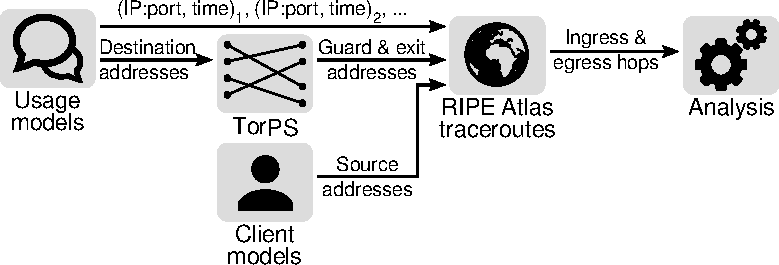
\includegraphics[width=\linewidth]{figures/simulations.pdf}
	\caption{The relation among our simulation components.  Our goal is to
	determine the ASes a Tor user's traffic traverses into and out of the Tor
	network.  Duplicate ASes on both sides can deanonymize streams.}
	\label{fig:simulations}
\end{figure}

In this analysis we assume that an AS that can see traffic entering the Tor network and 
DNS traffic at the other end can use this information in order to deanonymize the 
entering traffic. Here we seek to measure the chances an AS will be in the ``correct'' 
position to carry out such an attack.

A Tor exit can carry out DNS name resolution in two different ways: it can either do it
itself by running a name server locally, or it can rely on a 3rd-party name server, 
such as its ISP's name server or a public DNS name server like Google's 8.8.8.8.

Let us examine these two different scenarios: local resolution vs. 3rd-party 
resolution. With local resolution, a good position for an AS is to be on the path between 
a Tor client and a Tor guard and on the path between a Tor exit and any of the name 
servers the exit has to communicate with in order to resolve the name. These name servers 
can include the root name server, the TLD servers, and the other ones**fix this. The ASes 
along the way from the exit relay to the name servers will be able to see the domain 
names that are being queried.

For 3rd party resolution, a good position for an AS is to be on the path between 
a Tor client and a Tor guard and on the path between the exit relay and that 3rd party 
name server. Beyond that, the queries will look like they're coming from the IP address 
of the name server and not the IP address of the exit relay, which is what we're interested 
in.

\subsection{Learning AS-level paths}
In order to do our analysis, we need to have some way of figuring out the AS-level paths. 
We considered two options: the use of AS path inference and the use of traceroute data. 
We decided against AS path inference because Juen et al. showed that it can be quite
inaccurate~\cite{Juen2015a}.  Thus, we decided to go with actual traceroute data. Here,
again, we had to consider our options on how to obtain this data. We considered the
PlanetLab and RIPE Atlas measurement platforms and asking Tor relay operators to run
traceroutes for us.  We decided against using Tor relay operators to run traceroutes for
us because of the inconvenience (Murdoch paper did this and Juen paper did this). We
decided against PlanetLab because its nodes tend to be in university networks. Hence, we
decided to use RIPE Atlas~\cite{atlas}. RIPE Atlas has probes in many ASes that have Tor
relays. As shown in Table~\ref{tab:atlas-coverage}, for a day in May 2016, we found that
RIPE Atlas had probes in 52\% of ASes that contain Tor exit relays.  We found that RIPE
Atlas has probes in 51\% of ASes that contain Tor guard relays. More importantly, we found
that Atlas ASes cover 58\% of Tor exit bandwidth and 74\% of Tor guard bandwidth. This is
important because Tor relay usage is not evenly split among all of the relays. This
coverage is significant because as the Murdoch paper states, ``As Tor does not currently
implement a a mechanism for performing traceroutes, the operator of the node must do so
manually. Furthermore, the Juen paper was only able to cover around 28\% of exit bandwidth
by asking operators to run traceroutes for them.  Thus, we find that RIPE Atlas gives us a
great way to study the paths that Tor circuits might traverse. In order to get
our traceroutes, we ran traceroutes from probes that that were in the same ASes
as Tor guards and exits. \fixme{Mention why we picked AS 6128 as our client AS.}

% - 197 out of all 377 (52%) Tor exit ASes have Atlas probes.
% - 220 out of all 434 (51%) Tor guard ASes have Atlas probes.

% - Atlas ASes cover 57.53% of Tor exit bandwidth.
% - Atlas ASes cover 73.59% of Tor guard bandwidth.

\begin{table}[t]
	\caption{The coverage of RIPE Atlas nodes that are colocated with Tor guard and exit
	relays.}
	\label{tab:atlas-coverage}
	\centering
	\begin{tabular}{l|r r}
	\toprule
	\textbf{Atlas probe coverage} & \textbf{Tor guard ASes} & \textbf{Tor exit ASes} \\
	\midrule
	By bandwidth & 73.59\% & 57.53\% \\
	By number & 50.69\% & 52.25\% \\
	\bottomrule
	\end{tabular}
\end{table}

We also had to consider what method we would use to translate the IP addresses in
our traceroutes to ASes. The options we considered were Team Cymru~\cite{ipasn}
and pyasn~\cite{pyasn}. We decided to go with pyasn because it uses actual
control plane data in order to perform the translations vs. using whois, which
is what Team Cymru uses (find source for this).  (A word of caution: if there is
an AS that is annoucing bogons on a particular day, and you unluckily happen to
pick that day, you might get bogus translations. For example, an IP address like
10.10.10.1 might result in an AS number instead of 'None'.)

\subsection{Simulating Tor user activity}
In order to measure the chances an AS will be in the ``correct'' position to carry out a
deanonymization attack, we make use of TorPS, the Tor Path Simulator. This tool 
``faithfully mimics the behavior of Tor client software for creating exit circuits.''
That is, it gives us realistic combinations of guards and exits based on the state of the 
Tor network for a given time. TorPS is based on Tor version X. For each sample, it uses 
one guard which will expire after 270 days. We have TorPS simulate the behavior of a Tor 
client for the month of March 2016. We use 50,000 samples for the same reasons given in
``Users Get Routed.'' \fixme{Should we mention the fixes we made to TorPS? Should we mention 
the problem we found with their user models?} For our simulation, we had each sample 
visit domain.com\footnote{We redacted the real domain to anonymize our
submission.}---a website under our control---once per hour for the entire month
of March 2016.  Thus, each sample had a total of 744 opportunites to be
compromised (this assumes that the circuit changes every time the sample/user
visits domain.com).  It is much better to use a tool like TorPS in order to
measure these chances instead of just using all permutations of guard and exits.

In this analysis, we completely ignore caching of any type, so our results are overly 
pessimistic. \fixme{Mention that these results apply only to what we had data for: about 
half.}

Describe the four scenarios in the graph here: 1) Traditional, 2) Google, 3) Local, and 
4) Status Quo.

Traditional: ``Traditional'' represents the paths between all exit ASes that RIPE Atlas 
has coverage for and domain.com. That is, this measurement doesn't take DNS into account 
at all, as has been traditionally done.

Google (8.8.8.8): ``Google'' represents what would happen if all exit relays used 
Google's public DNS server for resolution. We ran traceroutes from probes in all the exit 
ASes that RIPE Atlas had coverage for to 8.8.8.8.

Local: ``Local'' represents what would happen if all exit relays ran their own name 
servers locally (e.g., the use of unbound) on their own machines. In order to figure out 
what ASes would be traversed on the way to resolve domain.com. In order to figure out the 
DNS delegation path, we use the command line option \texttt{+trace} of the
command line tool dig. Assuming no caching and assuming 
iterative resolution, for domain.com the name server will have to visit three name servers:
a root name server, a top level domain name server, and a second level domain name server. 

Status Quo: ``Status Quo'' represents to the best of our ability the type of name resolution 
that exit relays perform, whether that be their own or the use of 3rd-party name servers, 
which again includes public DNS name servers and their ISPs' name servers. To figure this 
out, we used the exitmap tool, our own website, and our own authoritative name server 
in order to figure out the IP addresses of the name servers that the exit relays were 
using. We then performed traceroutes from the exit ASes to the appropriate IP addresses 
in order to get the AS-level paths.

\fixme{Get the numbers from my data for the fan-out.}

As you can see in Figure~\subref{fig:compromised-streams} and
Figure~\subref{fig:time-until-compromise}, 
Google fared much better than the other situations. This might lead you to believe that 
Tor exit relays should use 8.8.8.8 for all of their name resolution needs, but then you've 
given Google A LOT of power. It might actually be better to tell Tor exit relay operators 
to use their ISPs' default name servers because the ISPs get to see the Tor destinations 
anyway!

The Status Quo results are significantly better than the Local results because only X\% 
of Tor exit relays actually do their own resolution.

\begin{figure}[t]
\centering
\subfigure[Number of compromised streams.]{
	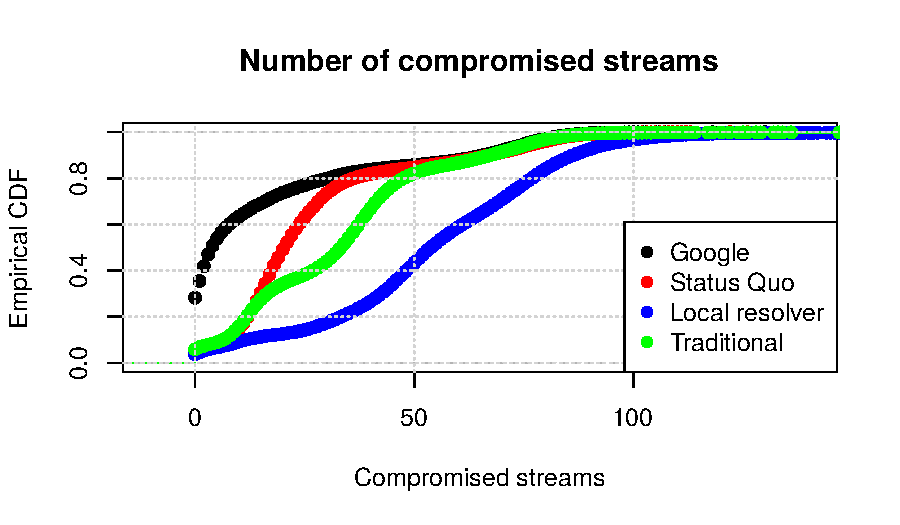
\includegraphics[width=0.6\linewidth]{figures/num-compromised-streams.pdf}
    \label{fig:compromised-streams}
}
\subfigure[Time to first compromise.]{
	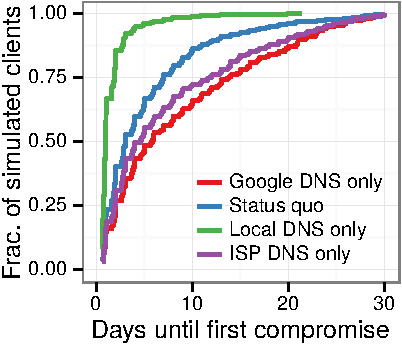
\includegraphics[width=0.6\linewidth]{figures/time-until-compromised.pdf}
    \label{fig:time-until-compromise}
}
\caption{Two simulations for March 2016 that show the number of compromised
	streams (Figure~\subref{fig:compromised-streams}) and the time until the
	first compromised stream (Figure~\subref{fig:time-until-compromise}).}
\label{fig:compromise-stream-time}
\end{figure}


\section{Discussion}
\label{sec:discussion}

In this section, we briefly discuss the ethics of our research, as well
as possible ways to defend against \name attacks.

\subsection{Ethics}
\label{sec:ethics}

Section~\ref{sec:load-freq} discusses how we set up an exit relay to
determine the number of DNS requests per five minute interval.  Since
our exit relay was forwarding traffic of Tor users, we contacted our
university's institutional review board (IRB) before running the
experiment.  Our IRB deemed that this research did not fall within the
realm of human subjects research.  In addition to contacting our IRB, we
adhered to The Tor Project's ethics guidelines~\cite{ethics-guidelines}.
Specifically, \first we ensured that we only collected data that is safe
to publish, \second we only collected data we needed, and \third we
limited the granularity of the data to minimize the likelihood of
reidentification.  The risk to Tor users of this experiment negligible.
As for the benefits, by conducting this experiment, we can improve our
understanding of the risks that DNS poses to the anonymity of Tor users
and use this understanding to improve protection for Tor users in the
future. Without this research, the design of defenses against \name
attacks would not be possible.  Thus, we believe that the benefits of
our experiment outweigh the risks.

\subsection{Defending against \name attacks}

We now discuss ways to defend against \name attacks.  We distinguish
between short-term solutions that can be implemented quickly
(Section~\ref{sec:short-term}), and long-term solution that need significantly more
work (Section~\ref{sec:long-term}).

\subsubsection{Short-term solutions}
\label{sec:short-term}

Operators of exist relays face a dilemma: they must either operate own
resolver, which exposes DNS queries to network adversaries; or, they
must use a third-party DNS resolver, which exposes DNS queries to a
third party.  Clearly, the goal is to minimize exposure of DNS requests,
but there are several dimensions to this.  In lieu of substantial DNS
protocol improvements, we can envision three extreme design points,
in which \emph{all} exit relays use \first Google's DNS resolver;
\second their own, local resolver; or \third the resolver provided by
their ISP.  Table~\ref{tab:setup-comparison}
summarizes the important tradeoffs for these three setups; the rest of
this section discusses these design points in more detail.

If all exit relays were to use Google's DNS resolver, the company would
obtain metadata about the activity of all Tor users, which runs counter to
Tor's design goal of distributing trust.  We clearly should avoid this
scenario. Note that, unfortunately, some of Tor's pluggable transports
have {\em already} made this design choice and should likely be updated
to mitigate user risk.  For example, Fifield \ea's~\cite{Fifield2015a}
Meek used Google's cloud infrastructure 
to reach the Tor network up until May 2016.
% died May 13, 2006. See https://lists.torproject.org/pipermail/tor-talk/2016-June/041699.html
Thousands of Meek clients
will thus select exit relays that use Google's DNS resolver, which means that Google
gets to see both traffic entering and, partially, exiting the Tor
network. 

Next, consider a Tor network that only uses local resolvers.  In this
case, Tor is fully independent of third-party resolvers, at the cost of
each iterative DNS query being exposed to a diverse set of ASes in the
network, allowing several parties to learn the DNS queries of Tor users.

Finally, all exit
relays could simply use their ISP-provided resolver.  This would minimize the
network exposure of DNS requests as resolvers are frequently in the same AS as
exit relays, and network-level adversaries would be unable to distinguish
between DNS requests from exit relays and unrelated ISP customers.  This
setup introduces the possibility of misconfigured and censored DNS
resolvers~\cite[\S~4.1]{Winter2014b}.  Besides, just a few ASes---OVH, for
example---host a disproportionate amount of exit relays, turning them into the
centralized data sinks that Tor aims to avoid.   

Considering the above, we believe that exit relay operators should avoid
public resolvers such as Google and OpenDNS.  Instead, they should
either use the resolvers provided by their ISP, or run their own,
particularly of the operator's 
ISP already hosts many other exit relays.  Local
resolvers can further be optimized to minimize information leakage,
by (for example) enabling QNAME minimization~\cite{qname-minimization}. 

\begin{table}[t]
  \renewcommand{\tabcaptext}{A comparison between three design points for DNS
          resolver configuration, assuming all Tor exit relays use the
          setup in question.  Solid black circles are most desirable.}
	\topcap{\tabcaptext}
	\centering
	\begin{tabular}{l c c c}
	\toprule
	\textbf{Setup} &
	\begin{tabular}{@{}c@{}}\textbf{Network-level}\\\textbf{Protection}\end{tabular} &
	\begin{tabular}{@{}c@{}}\textbf{Avoiding}\\\textbf{Centralization}\end{tabular} &
	\begin{tabular}{@{}c@{}}\textbf{Response}\\\textbf{Quality}\end{tabular} \\
	\midrule
	All Google & \RIGHTcircle & \Circle & \CIRCLE \\
	All Local & \Circle & \CIRCLE & \CIRCLE\\
	All ISP & \CIRCLE & \RIGHTcircle & \RIGHTcircle \\
	\bottomrule
	\end{tabular}
	\bottomcap{\tabcaptext}
       \label{tab:setup-comparison}
\end{table}

In addition to making recommendations to exit relay operators, we can
remotely influence the cache of each exit relay's resolver.  For
example, using {\tt exitmap}, we can resolve potentially sensitive DNS
domain names over each exit relay continuously, right before its TTL is
about to expire.  In such a setup, an attacker gains no advantage from
observing DNS traffic from the exit relays is always in every exit
relay's DNS resolver cache.  This approach may not scale, considering
the potentially large number of domain names that would need to be
cached (recall that the long tail of unpopular sites are most vulnerable
to \name attacks), but it allows us to eliminate DNS-based correlation
attacks for a select number of sites.

Finally, Tor can fix the Tor clipping bug and consider significantly increasing the
minimum TTL for the DNS cache at exits to make \name attacks less precise.
This adjustment requires finding the longest acceptable TTL that does not have a
notable negative detriment to user experience.

\subsubsection{Long-term solutions}
\label{sec:long-term}

Additional practical defenses are on the horizon.  Zhu \ea~\cite{Zhu2015a} proposed
T-DNS, which employs several TCP optimizations to transport the DNS protocol
over TLS and TCP.  Since T-DNS is based on TCP, Tor can transport tehse queries.
The TLS layer provides confidentiality between exit relays and their resolvers.
Finally, site operators whose users are particularly concerned about 
safety should offer an onion service as an alternative.  Facebook, for example,
set up \url{facebookcorewwwi.onion}.  When
connecting to the onion service, Tor users never leave the Tor network, and
hence no not need DNS.

Deploying defenses against website fingerprinting attacks in Tor should be an
important long-term goal, as well.
Although growing the Tor network will help defend against website
fingerprinting attacks to some degree, the most important change is to
deploy defenses against these attacks in the first place.  Since website
fingerprinting attacks significantly increase precision, defenses should
be designed to significantly reduce the recall of these attacks, even at
the expense of precision.



\section{Conclusion}
\label{sec:conclusion}
\begin{itemize}
	\item Lack of diversity in DNS resolvers is concerning.
\end{itemize}


\section*{Acknowledgments}
This research was supported in part by the Center for Information Technology
Policy at Princeton University.
We want to thank Jed Crandall for providing infrastructure for our measurements.
Thanks to Aaron Johnson for helpful feedback.


\balance
\bibliographystyle{IEEEtranS}
\bibliography{references}

\end{document}
